\documentclass[xcolor=dvipsnames]{beamer}
%\usepackage[OT4]{fontenc}
%\usepackage[utf8]{inputenc}
%\usepackage[polish]{babel}
\usepackage{fancyvrb}
\usepackage{thumbpdf}
\usepackage{relsize}
\usepackage{amsmath}
\usepackage{pgfplots}

\useinnertheme[shadow]{rounded}
\useoutertheme[right,width=2cm,hideothersubsections]{sidebar}

\definecolor{ZooplusGreen}{RGB}{129,197,46}
\definecolor{ZooplusOrange}{RGB}{255,136,0}
\definecolor{ZooplusSeriesGreen1}{RGB}{106,163,38}
\definecolor{ZooplusSeriesGreen2}{RGB}{129,197,46}
\definecolor{ZooplusSeriesGreen3}{RGB}{186,219,164}
\definecolor{ZooplusGrey}{RGB}{64,64,64}
\setbeamercolor{structure}{fg=ZooplusGreen}
\setbeamercolor{palette primary}{fg=ZooplusGrey,bg=ZooplusSeriesGreen3}
\setbeamercolor{palette secondary}{fg=ZooplusGrey,bg=ZooplusSeriesGreen2}
\setbeamercolor{palette tertiary}{fg=ZooplusGrey,bg=ZooplusSeriesGreen1}
\setbeamercolor{palette quaternary}{fg=ZooplusGrey,bg=ZooplusGreen}
\setbeamercolor{titlelike}{parent=palette quaternary}
\setbeamercolor{block title}{fg=ZooplusGrey,bg=ZooplusGreen}
\setbeamercolor{block title alerted}{use=alerted text,fg=ZooplusGrey,bg=alerted text.fg!75!bg}
\setbeamercolor{block title example}{use=example text,fg=ZooplusGrey,bg=example text.fg!75!bg}
\setbeamercolor{block body}{parent=normal text,use=block title,bg=block title.bg!25!bg,fg=ZooplusGrey}
\setbeamercolor{block body alerted}{parent=normal text,use=block title alerted,bg=block title alerted.bg!25!bg}
\setbeamercolor{block body example}{parent=normal text,use=block title example,bg=block title example.bg!25!bg}
\setbeamercolor{sidebar}{bg=ZooplusGreen!70}
\setbeamercolor{palette sidebar primary}{fg=ZooplusGrey}
\setbeamercolor{palette sidebar secondary}{fg=ZooplusGrey!90}
\setbeamercolor{palette sidebar tertiary}{fg=ZooplusGrey!80}
\setbeamercolor{palette sidebar quaternary}{fg=ZooplusGrey!70}
\setbeamercolor*{separation line}{}
\setbeamercolor*{fine separation line}{}
\logo{
\includegraphics[scale=0.25]{../../zooplus_logo.png}}

\usefonttheme{default}
\setbeamercovered{transparent}
\title{Akka -- actors system for Scala \& Java}
\author{Jacek~Bilski}
\date{\today}
\subject{Akka -- actors system for Scala \& Java}

\setbeamertemplate{navigation symbols}
{
	\usebeamercolor[fg]{navigation symbols dimmed}
	{
		\insertframenumber\,/\,\inserttotalframenumber
	}
}

\begin{document}

\begin{frame}
\titlepage
\end{frame}

\begin{frame}
\frametitle{Agenda}
\tableofcontents[pausesections]
\end{frame}

\section{Scala}

\frame[containsverbatim]{
\frametitle{Scala's Hello World!}
\begin{Verbatim}[obeytabs=true,fontsize=\relscale{0.7},tabsize=2]
package com.zooplus.jacekb.learningTime.scala

object Hello {
	def main(args: Array[String]) {
		val name = "Zooplus"
		println(s"Hello World! Hello $name!")
	}
}
\end{Verbatim}
}

\begin{frame}
\frametitle{Hello World explained}
\begin{itemize}
\item One method defined (Scala's equivalent of Java's $main$ method), which just prints the usual ''Hello World!''.
\item No semicolon at the end, we rarely need them.
\item No ''return'' keyword, value of last expression is the function's result.
\item Variables and parameters are defined in a different way that in Java: $name:\:Type$
\item Generics are using square brackets ($[]$) rather than lesser/greater than ($<>$)
%\item Hello is an object, not a class. It's a singleton with all methods ''static''. There are no ''static'' methods in Scala, you define a class and object with the same name.
\end{itemize}
\end{frame}

\begin{frame}
\frametitle{Hello World explained -- continued}
\begin{itemize}
\item We define functions with: $def\:functionName$,
\item then we add some parameters: $def\:f(x:\:Int, y:\:String)$,
\item then we may (it's necessary only for recursive functions) define return type: $def\:f(x:\:Int):\:Int$,
\item then we define functions body: $\{ x * x \}$. %(we can omit parenthesis, because the body is a proper Scala expression).
%\item In total: $def\:f(x:\:Int) \{ x * x \}$.
%\item When function doesn't take parameters, we can skip the parenthesis completely: $def\:f = 3$.
\item In method's body we can define a variable using $val\:variableName = value$.
\item Types of variables can usually are inferred, usually can be omitted.
\end{itemize}
\end{frame}


\section{Actors system}

\subsection{Akka}

\begin{frame}
\frametitle{Akka}
\begin{itemize}
\item \href{http://akka.io/}{http://akka.io/}
\item Implements actors system for Scala \& Java
\item Based on Erlang actors
\end{itemize}
\end{frame}

\subsection{Actors systems}

\begin{frame}
\frametitle{Actors system}
\begin{itemize}
\item Hierarchy of actors
\item Manages actors, creates threads, routes messages, etc.
\end{itemize}
\end{frame}

\subsection{Actors}

\begin{frame}
\frametitle{Actors}
Main goal: solve several issues with concurrency, parallelism or multithreaded programming
\begin{itemize}
\item Very lightweight concurrent entities
\item Process messages asynchronously, one by one using an event-driven receive loop
\item No need to worry about threads, locks, etc. if messages are immutable
\item Can be transparently remote
%\item ''Little'' SOA
\item Realization of an idea behind OOP -- objects exchanging messages
\end{itemize}
\end{frame}


\section{Problem}

\subsection{Problem}

\begin{frame}
\frametitle{Problem: calculating value of $\pi$}
Formula:
%\begin{equation}
\[\sum_{n=0}^\infty \frac{(-1)^n}{2n+1} = 1 - \frac{1}{3} + \frac{1}{5} - \frac{1}{7} + \ldots = \frac{\pi}{4}\]
%\end{equation}
\end{frame}

\subsection{Solution}

\begin{frame}
\frametitle{Divide and conquer}
\begin{itemize}
\item Problem is easily parallelizable,\ldots
\item \ldots{}so we split calculations in chunks and calculate in different actors.
\end{itemize}
\end{frame}

\begin{frame}
\frametitle{Solution overview}
\begin{tikzpicture}
\end{tikzpicture}
\end{frame}

\frame[containsverbatim]{
\frametitle{App}
\begin{Verbatim}[obeytabs=true,fontsize=\relscale{0.7},tabsize=2]
def calculate(workersNo: Int, elementsNo: Int, messagesNo: Int) {
	// Create an Akka system
	val system = ActorSystem("PiSystem")

	// create the result listener, which will print the result and
	// shutdown the system
	val listener = system.actorOf(Props[Listener], name = "listener")

	// create the master
	val master = system.actorOf(Props(new Master(
		workersNo, messagesNo, elementsNo, listener)),
		name = "master")

	// start the calculation
	master ! Calculate
}

calculate(workersNo = 4, elementsNo = 10000, messagesNo = 100000)
\end{Verbatim}
}

\frame[containsverbatim]{
\frametitle{Listener}
\begin{Verbatim}[obeytabs=true,fontsize=\relscale{0.8},tabsize=2]
class Listener extends Actor {
def receive = {
	case PiApproximation(pi, duration) =>
		println(s"\tPi approximation: \t$pi)
		println(s"\tCalculation time: \t$duration")
		context.system.shutdown()
}}
\end{Verbatim}
}

\frame[containsverbatim]{
\frametitle{Master}
\begin{Verbatim}[obeytabs=true,fontsize=\relscale{0.7},tabsize=2]
class Master extends Actor {

var pi: BigDecimal = 0
val start: Long = System.currentTimeMillis
var nrOfResults: Int = _
val workerRouter = context.actorOf(
	Props[Worker].withRouter(RoundRobinRouter(nrOfWorkers)),
		name = "workerRouter")

def receive = {
	case Calculate =>
		for (i <- 0 until nrOfMessages)
			workerRouter ! Work(i * nrOfElements, nrOfElements)
	case Result(value) =>
		pi += value
		nrOfResults += 1
		if (nrOfResults == nrOfMessages) {
			// Send the result to the listener
			listener ! PiApproximation(pi,
					duration = (System.currentTimeMillis - start).millis)
			context.stop(self) // Stops this actor and all its children
		}
}}
\end{Verbatim}
}

\frame[containsverbatim]{
\frametitle{Worker}
\begin{Verbatim}[obeytabs=true,fontsize=\relsize{-2},tabsize=2]
class Worker extends Actor {

def calculatePiFor(start: Int, nrOfElements: Int): BigDecimal = {
	var acc = 0.0
	for (i <- start until (start + nrOfElements))
		acc += 4.0 * (1 - (i % 2) * 2) / (2 * i + 1)
	acc
}

def receive = {
	case Work(start, nrOfElements) =>
		// perform the work
		sender ! Result(calculatePiFor(start, nrOfElements))
}}
\end{Verbatim}
}

\subsection{Results}

\begin{frame}
\frametitle{Results}
$\pi = 3.141592652589784499499528724894 \gets$ no wonder :)
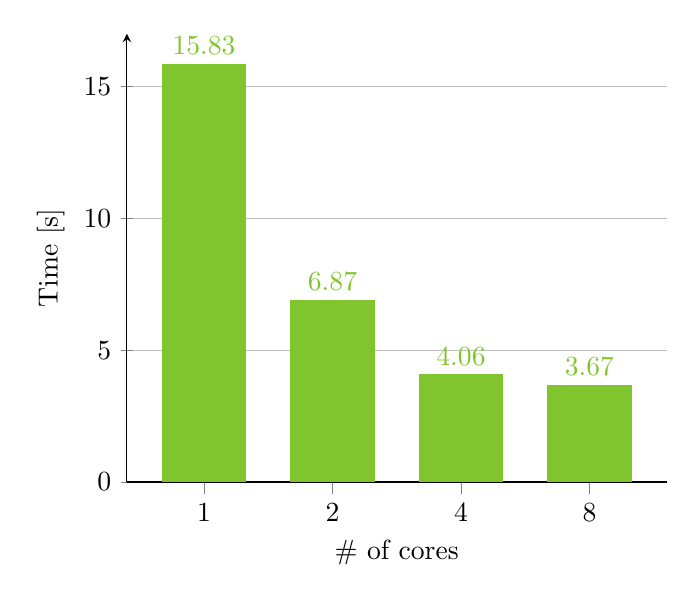
\begin{tikzpicture}
\begin{axis}[
	ylabel={Time [s]},
	ybar,
	xlabel={\# of cores},
	symbolic x coords={1,2,4,8},
	xtick=data,
	enlarge x limits=0.2,
	nodes near coords,
	bar width=30pt,
	grid=none,
	ymajorgrids=true,
	axis x line*=bottom,
	axis y line=left,
	ymin=0,
	ymax=17,
]
\addplot[color=ZooplusGreen, fill=ZooplusSeriesGreen2] coordinates {(1,15.830) (2,6.871) (4,4.063) (8,3.668)};
\end{axis}
\end{tikzpicture}
%Execution times:\\
%1 worker -- 15830 milliseconds\\
%2 workers -- 6871 milliseconds\\
%4 workers -- 4063 milliseconds\\
%8 workers -- 3668 milliseconds
\end{frame}


\section{Why all that?}

\begin{frame}
\frametitle{Why all that?}
\begin{itemize}
\item Scalability (both horizontal and vertical)
\item Fault tolerance -- hierarchies and supervision
\item Load management -- back-off strategies, timeouts, processing isolation
\item Batch processing in a ''divide and conquer'' way
\item Highly responsive systems
\item Asynchronous message processing
\end{itemize}
\end{frame}

\begin{frame}
\frametitle{There's more!}
Akka is extensible:
\begin{itemize}
\item Camel integration,
\item clustering,
\item durable mailboxes,
\item OSGi support,
\item MQ systems support
\item \ldots and many more
\end{itemize}
\end{frame}

\section{Questions?}

\begin{frame}
\frametitle{Questions?}
\begin{center}
\Huge{?}
\end{center}
\end{frame}

\end{document}
